\tableofcontents

\section{Introdução}\label{introduuxe7uxe3o}

A interação entre componentes de um sistema que possuem regras simples
leva a formação de padrões complexos e características como emergência,
livre de escala e heterogeneidade. Fenômenos emergentes são presentes em
sistemas complexos e caracterizados pelo resultado espontâneo da
interação entre os milhares de componentes que constituem o sistema. Um
grande exemplo de emergência ocorre durante a noite do sudeste asiático,
quando vagalumes da região piscam de acordo ajustam a frequência do
piscar de suas luzes de acordo com os vizinhos mais próximos, até que o
efeito seja extendido por todo o sistema, de forma que os indivíduos
pisquem em sincronia \cite{johnson2002emergence}.

No contexto de dinâmicas sociais, isto é, modelos matemáticos que buscam
reproduzir o comportamento humano em redes, a emergência pode ser
caracterizada como um fenômeno relacionado a polarização
\cite{maia2021emergence}. Aqui e no restante do relatório, definimos
polarização como a fragmentação de opiniões, um estado contrário ao
consenso. Diversos estudos mostram que a polarização pode ter profunda
influência no âmbito político, como visto nas manifestações
anti-democráticas e violentas ocorridas em Brasília no dia 8 de Janeiro
de 2023 \cite{interian2023polarization,layton2021polarization}. Dessa
forma, é de suma importância estudar a polarização para evitar que
cenários de discórdia se repitam.

A física estatística desenvolveu ferramentas para o estudo de sistemas
de muitas partículas interagentes, os quais são adaptados com facilidade
para o estudo de dinâmicas sociais. Ersnt Ising encontrou a solução
exata para um modelo de paramagneto, representando materiais que podem
alcançar dois estados conflitantes e buscam um estado de mínima energia.
O modelo recebeu o nome de Ising e pode ser considerado como um modelo
para simples opiniões, onde há uma transição de fase entre os estados de
polarização e consenso. O modelo de Sznajd foi inspirado pelo primeiro
modelo e busca explorar como opiniões semelhantes são necessárias para
influenciar outros. Já o modelo votante ilustra como a maioria pode
influenciar vizinhos, explorando por sua vez como a ordem emerge a
partir da opinião maioria.

Para uma compreensão mais realista do fenômeno do consenso, é crucial
simular esses modelos em diferentes topologias de rede, uma vez que ela
desempenha um papel fundamental na dinâmica do consenso e na polarização
resultante. Estudos recentes destacam a influência significativa da
topologia da rede nos resultados de consenso e polarização
\cite{pineda2023machine}. Dada a significativa influência da topologia
da rede na formação de consenso, surge a necessidade de explorar a
viabilidade de um modelo de Aprendizado de Máquina para prever variáveis
dinâmicas de sistemas com base nas propriedades de rede subjacente. Essa
abordagem, amplamente aplicada em campos como sincronização e
disseminação de epidemias \cite{rodrigues2019machine}, levanta a questão
sobre sua aplicabilidade no estudo do modelo de Sznajd. Este trabalho
investiga essa possibilidade, focalizando na capacidade do aprendizado
de máquina de antecipar variáveis dinâmicas do modelo de Sznajd, com
base na topologia da rede. Destaca-se assim, o potencial dessas análises
de rede para a compreensão de sistemas dinâmicos, fornecendo
\textit{insights} valiosos sobre a emergência e evolução da polarização
na sociedade.

Esse trabalho apresenta valiosos \emph{insights} na relação entre
topologia de rede e dinâmicas sociais, destacando o potencial do uso de
métricas de rede para análise de sistemas dinâmicos. Visto a alta
colinearidade nas métricas de caracterização \ref{figure:2} e
comportamento das variáveis resposta, uma metodologia baseada em
\emph{Forward Selection} e Regressão não Linear foi proposta, garantindo
alta acurácia, robustez e maior explicabilidade em relação a
\emph{Random Forests}.

\section{Materiais e Métodos}\label{materiais-e-muxe9todos}

\subsection{Geração de Redes
Aleatórias}\label{gerauxe7uxe3o-de-redes-aleatuxf3rias}

Seis diferentes topologias das redes foram examinadas. As redes
Erdös--Rényi, Barabási--Albert linear, Barabási--Albert não linear com
\(\alpha=0.5\) and \(\alpha=1.5\), Watts--Strogatz e Waxman
\textasciitilde{}\cite{boccaletti2006complex,costa2007characterization}.
Essas topologias buscam abordar diferentes estruturas que sociedades
reais possam admitir, considerando a presença de hubs, comunidades e
\emph{small-world}. Ou seja, como as redes geradas por esses modelos
apresentam diferentes propriedades que podems ser controladas através de
seus parâmetros, poderemos gerar um banco de dados com exemplos de
topologias diferentes. Assim, os efeitos de propriedades topológicas no
processo dinâmico podem ser verificados, visto que muitas propriedades,
como distância entre os vértices ou nível de centralidade, sofrerão
variações nas bases geradas. Essa variação é importante para oferecermos
exemplos diferentes aos modelos de aprendizado que usaremos na fase de
predição das variáveis dinâmicas. Para cada uma dessas redes, 100
instâncias foram criadas visando diminuir efeitos da aleatoriedade na
construção do modelo.

\subsubsection{Erdos-Renyi (ER)}\label{erdos-renyi-er}

O modelo de Erdos-Renyi (ER) é um dos mais estudados e detalhados na
teoria dos grafos. É formado ao ligar \(N\) nós entre as possíveis
arestas com probabilidade \(p\). Apesar de não representar com
fidelidade cenários do mundo real, possui apelo matemático por possuir
características bem definidas.

\subsubsection{Small-World de Watts e
Strogatz}\label{small-world-de-watts-e-strogatz}

Diversas redes do mundo real exibem a propriedade \emph{small-world},
isto é, a maioria dos vértices podem ser alcançados pelo restante a
partir de um pequeno número de arestas. Essa propriedade é muito comum
em redes sociais.

Outra propriedade muito relevante em redes é a presença de \emph{loops}
de tamanho três: se \(i\) está conectado a \(j\) e \(k\), há uma grande
probabilidade que \(j\) e \(k\) estejam conectados por sua vez. As redes
ER possuem característica de pequeno mundo, porém não apresentam muitos
triângulos. De forma contrária, é fácil construir redes com abundância
de loops, mas é difícil garantir a presença de características de
pequeno mundo.

O modelo mais popular que uniu as duas características foi desenvolvido
por Watts e Strogatz e recebeu o nome de modelo \emph{small-world} de
Watts-Strogatz (WS). Para construí-lo, comece com uma grade triangular e
realize a reconexão de cada aresta presente com probabilidade \(p\).
Para \(p\approx 0\), a rede original é mantida, enquanto que para
\(p\approx 1\) há uma rede aleatória.

\begin{figure}
\centering
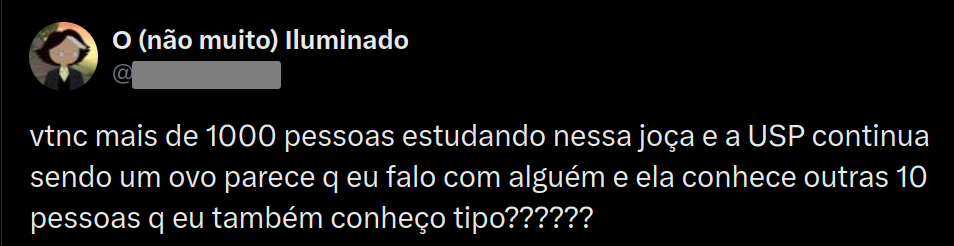
\includegraphics[width=4.16667in,height=\textheight]{tweet_SW.png}
\caption{Post na plataforma X (Twitter) discorre sobre a rede de
interações da Universidade de São Paulo, a qual possui características
estudadas por Watts e Strogatz. Acessado em 03/11/2024 em
https://x.com/LuzMadLED/status/1852872862903771258}
\end{figure}

\subsubsection{Redes Livre de Escala de Barabási e
Albert}\label{redes-livre-de-escala-de-barabuxe1si-e-albert}

Barabási e Albert demonstraram que a distribuição do grau de inúmeros
sistemas do mundo real é caracterizada por uma distribuição assimétrica.
Nessas redes, alguns vértices são altamente conectados enquanto outros
possuem poucas conexões. Uma característica muito importnate dessa rede
é a existência de \emph{hubs}, vértices que são conectados a uma fração
significativa do total da rede. A construção das redes Barabási-Albert
inicia com um conjunto de vértices e iterativamente adiciona arestas de
forma que os vértices mais conectados possuam maior chance de formar
novas arestas.

\subsubsection{Redes Geográficas}\label{redes-geogruxe1ficas}

A maioria das redes complexas mora em um espaço abstrato, onde a posição
dos vértices não tem um sentido particular. Em algumas redes, porém, a
posição dos vértices pode ter importante impacto, como por exemplo, no
caso de redes de transporte rodoviário, aéreo e redes neuronais. Esses
exemplos recebem o nome de redes geográficas. Uma maneira simples de
gerar redes geográficas é distribuir \(N\) vértices em um espaço
abstrato e conectá-los com uma probabilidade que decai de acordo com a
distância entre eles.

\subsection{Simulação de Monte Carlo do modelo de
Sznajd}\label{simulauxe7uxe3o-de-monte-carlo-do-modelo-de-sznajd}

O modelo de \emph{spin} de Ising é um dos modelos mais utilizados na
mecânica estatística\textasciitilde{}\cite{castellano2009social}. No
artigo \cite{sznajd2000opinion} é proposto o modelo de Sznajd, uma
adaptação de Ising para descrever dinâmicas de opinião em uma
comunidade.

O modelo original segue uma simulação estocástica implementando o
fenômeno de validação social nos agentes \(S_i, i=1,2,...,N\) com
opiniões \(O=\{-1, +1\}\). A cada passo, dois vizinhos são selecionados
e o sistema é atualizado de acordo com as seguintes regras dinâmicas:

\begin{itemize}
\tightlist
\item
  Se \(SiS_{i+1}=1\), então os vizinhos \(S_{i-1}\) e \(S_{i+2}\)
  recebem a opinião do par \(S_i, S_{i+1}\)
\item
  Se \(SiS_{i+1}=-1\), então \(S_{i-1}=S_{i+1}\) e \(S_{i+2}=S_i\)
\end{itemize}

O modelo original foi proposto para um sistema unidimensional. \% No
entanto, a dinâmica foi modificada de forma incluir uma rede
complexa\textasciitilde{}\cite{sanchez2004sznajd}. \% Nesse trabalho
será utilizada a adaptação apresentada em \cite{Bernardes_2002} para
implementação do modelo de Sznajd em redes com duas opiniões. Considere
uma rede de \(N\) pessoas, com opiniões \(O =\{-1, +1\}\) inicialmente
distribuidas de forma aleatória. Cada indivíduo é uma variável dinâmica
binária \(s(x, t)=O\) de grau \(k_x\), em que \(x=1,...,N\). Uma
iteração \(t\) de uma sequência de iterações até o consenso é descrita
abaixo:

\begin{itemize}
\tightlist
\item
  Uma dupla de nós vizinhos \(i\) e \(j\) é escolhida aleatoriamente
\item
  Se \(s(i, t) \ne s(j, t)\) a iteração termina
\item
  Se \(s(i, t) = s(j, t)\), a união dos vizinhos de \(i\) e \(j\) recebe
  a opinião de \(i\).
\end{itemize}

\subsubsection{Variáveis dinâmicas de
interesse}\label{variuxe1veis-dinuxe2micas-de-interesse}

O \textbf{tempo de consenso}, definido como o período necessário para
que o sistema alcance um estado estacionário, é uma métrica crucial na
análise da dinâmica de consenso, bem como a \textbf{frequência da troca
de opinião}. Durante a simulação, registramos tanto o tempo de consenso
quanto a frequência de troca de opinião como indicadores-chave do
comportamento do sistema. O histograma de ambas variáveis aleatórias são
exibidos abaixo com a estimativa de densidade correspondente. Se faz
necessária a utilização da escala log para visualização devido ao
aspecto de cauda longa das distribuições.

\begin{figure}
\centering
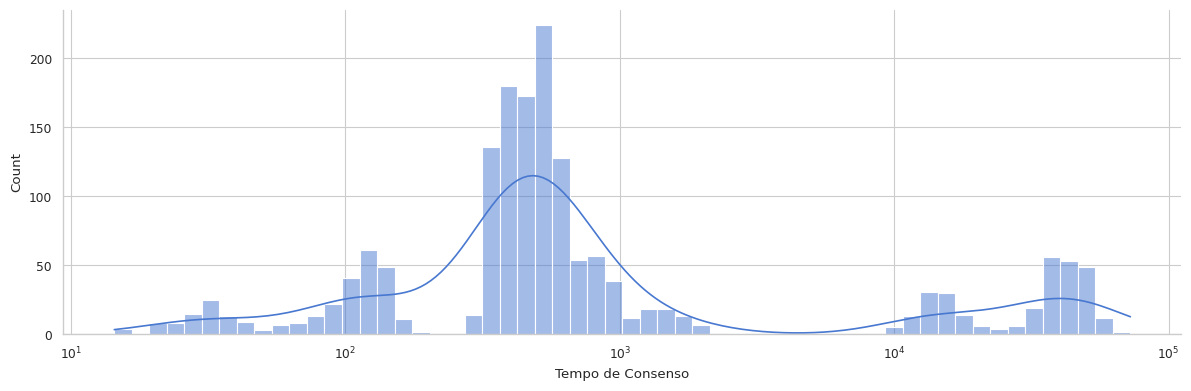
\includegraphics[width=6.25in,height=\textheight]{consensus_hist.png}
\caption{Histograma do Tempo de Consenso na escala logarítmica}
\end{figure}

\begin{figure}
\centering
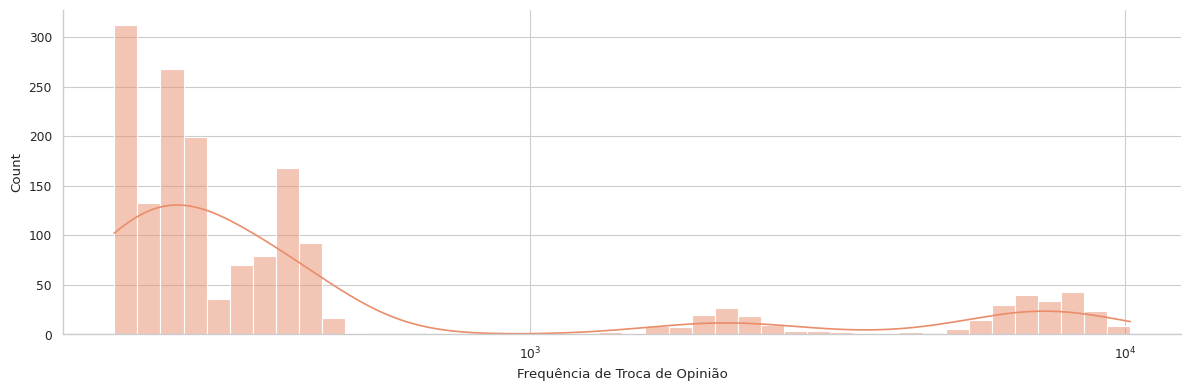
\includegraphics[width=6.25in,height=\textheight]{frequency_hist.png}
\caption{Histograma da Frequência de Troca de Opinião na escala
logarítmica}
\end{figure}

\subsubsection{Inicialização dos
nós}\label{inicializauxe7uxe3o-dos-nuxf3s}

Os parâmetros para as redes e o modelo foram fixados para proporcionar
um patamar conciso durante os testes com os algoritmos de aprendizado de
máquina. Ao fixar esses parâmetros é possível focar no impacto de outras
variáveis na análise. Dessa forma, as simulações contarão com as redes
com um número de nós fixo, a saber, \(N=1000\), além de uma porcentagem
de nós com opiniões positivas \(p = 0,2\).

Além disso, adotamos três abordagens distintas de inicialização para os
nós com opiniões positivas nas simulações. Primeiramente, a
inicialização aleatória, atribuindo aleatoriamente opiniões positivas
aos nós. Em seguida, adotamos a estratégia de inicialização inversa, na
qual os nós com menor grau receberão opiniões positivas. Por fim,
aplicaremos a inicialização direta, na qual os nós mais influentes na
rede receberão opiniões positivas. É de suma importância simular o
sistema com diferentes inicializações, possibilitando analisar como a
importância das \emph{features} são influenciadas em cada caso e
compreender melhor como situações de consenso podem ser favorecidas.

\subsection{Caracterização de
Redes}\label{caracterizauxe7uxe3o-de-redes}

Buscamos caracterizar cada rede \(i\) utilizando um vetor de features
derivado de sua estrutura e denotado por
\(X_i=\{X_{i1}, X_{i2}, ...,X_{ik}\}\), em que \(X_{ik}\) é a k-ésima
métrica da rede \(i\). Assim, foram utilizadas diversas medidas,
incluindo o coeficiente de \emph{clustering}, \emph{closeness
centrality}, \emph{betweenness centrality}, \emph{average shortest path
lenght}, coeficiente de correlação de Pearson do grau, \emph{information
centrality}, \emph{approximate current flow betweenness centrality} e
\emph{eigenvector centrality}, Entropia de Shannon e segundo momento do
grau. Tais medidas, usadas coletivamente aqui, fornecem \emph{insights}
valiosos sobre a topologia, conectividade, eficiência, influência e
organização em redes complexas \cite{costa2007characterization}.

\begin{figure}
\centering
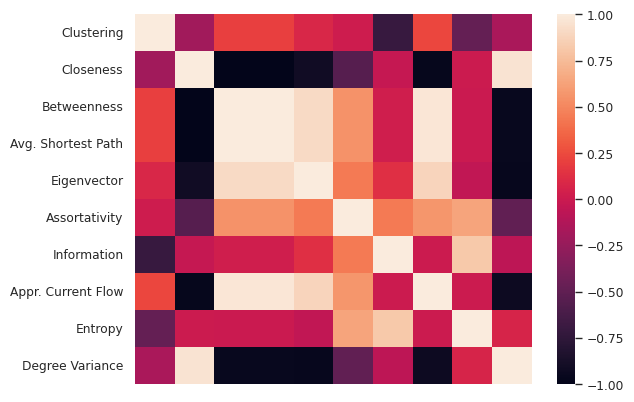
\includegraphics[width=\textwidth,height=2.66667in]{heatmap.png}
\caption{\emph{Heatmap} utilizando correlação de Spearman entre as
features. É possível observar alta colinearidade entre diversas
medidas.}
\end{figure}

Podemos dividir as métricas descritas acima entre três grandes grupos,
sendo eles medidas de centralidade (\emph{closeness centrality},
\emph{betweenness centrality}, \emph{average shortest path lenght},
\emph{information centrality}, \emph{approximate current flow
betweenness centrality} e \emph{eigenvector centrality}), de
transitividade (\emph{clustering}) e de conectividade (Assortatividade,
Entropia de Shannon e segundo momento do grau). Podemos obter um
\emph{heatmap} entre as features obtidas para as redes geradas
utilizando a correlação de Spearman, uma medida que quantifica a
colinearidade entre duas variáveis. Ao analisar o \emph{heatmap}, vemos
que há grande correlação linear entre diversas feautres, principalmente
aquelas que pertencem aos mesmos grupos. Esse resultado é importante
pois quando há informação mútua entre variáveis, o grau de influência no
resultado de modelos de Aprendizado de Máquina é diluído.

A seguir, realizamos uma revisão das métricas de rede mais importantes
para compreensão desse trabalho.

\subsubsection{\texorpdfstring{\emph{Closeness
Centrality}}{Closeness Centrality}}\label{closeness-centrality}

Em redes, quanto mais próximo a outros um vértice está, maior a sua
importância na rede. Assumindo que as interações entre nós seguem o
caminho mais curto, a \emph{Closeness Centrality} de um nó \(u\) é
definida como o recíproco da distância do caminho mais curto entre \(u\)
e os outros \(n-1\) nós da rede \(v=1,...,n\).

\[
CC(u) = \dfrac{n-1}{\sum_v d(u, v)}
\]

Onde \(d(u, v)\) é a distância do caminho mais curto entre \(v\) e
\(u\). Quanto maior o valor de \emph{Closeness}, maior a importância do
vértice na rede. Para caracterizar a rede foi utilizada o
\emph{Closeness} médio dos nós.

\subsubsection{\texorpdfstring{Coeficiente de
\emph{Clustering}}{Coeficiente de Clustering}}\label{coeficiente-de-clustering}

Uma maneira simples de caracterizar a presença de \emph{loops} de
tamanho três é através do coeficiente de \emph{Clustering}. \[
C = 3\frac{\#\text{triângulos}}{\#\text{tríades}}
\]

O fator 3 leva em conta que cada triangulo pode ser parte de três
triplas diferentes, cada uma com um vértice sendo o principal e garante
que \(C \in [0, 1]\).

\subsubsection{Entropia de Shannon}\label{entropia-de-shannon}

Entropia é um conceito chave em termodinâmica, mecânica estatística e
teoria da informação e está relacionada fisicamente com a quantidade de
disordem e informação presentes em um sistema. Na teoria ade informação,
entropia descreve quanta aleatoriedade está presente em um evento
aleatório. Esse conceito pode ser aplicao para o estudo de redes
complexas ao calcular a entropia da distribuição do grau. Essa medida
provê uma média de heterogeneidade da rede e pode ser definida como

\[
H = - \sum_k P(k) \log P(k)
\]

O valor máximo de entropia é obtido para uma distribuição uniforme
quando todos vértices possuem o mesmo grau e está relacionada com a
robustez e resiliência da rede.

\subsubsection{Assortatividade}\label{assortatividade}

Uma característica muito importante em redes é a presença de conexões
homogeneas. Podemos nos perguntar, por exemplo, quão provável é a
conexão entre nós similares. A assortatividade mede a similaridade de
conexões no grafo com respeito ao grau do nó. Quando vértices de alto
grau tendem a se conectar com vértices de alto grau, a rede é
assortativa. Por outro lado, se os vértices de alto grau se conectam
vértices de baixo grau a rede é disassortativa.

\textbackslash cite newman assortativity mixing

O cálculo da assortatividade é feito através do Coeficiente de
Correlação de Pearson \(r\). Caso \(r>0\), a rede é assortativa; se
\(r<0\), a rede é disassortativa; para \(r=0\) não existe relação entre
o grau dos vértices.

\subsection{Aprendizado de Máquina}\label{aprendizado-de-muxe1quina}

Nesse trabalho assumimos que o tempo para alcançar consenso \(Y_i\) e a
frequência de mudança de opinião \(C_i\) podem ser inferidos a partir do
vetor de \emph{features} \(X_i\). A explicação abaixo foca na predição
de \(Y_i\) mas também é válida para \(C_i\).

\[
Y_i = f(X_i)+\delta
\]

Nosso objetivo é encontrar a função \(f\) que relaciona \(Y_i\) às
métricas da rede. Trataremos predição de \(Y_i\) como um problema de
regressão em que \(\delta\) é um termo que representa uma distribuição
normal com média zero e desvio padrão \(\sigma\). Esse termo representa
a incerteza nos dados, que incluem as medidas que não foram incluídas no
modelo e as flutuações aleatórias na simulação das redes e modelos.

\subsubsection{Coeficiente de Determinação
(R2)}\label{coeficiente-de-determinauxe7uxe3o-r2}

O coeficiente de determinação, \(R^2\), é uma métrica usada para medir o
quão bem um modelo de regressão se ajusta aos dados
\cite{johnson2017r2}.

\[
R^2=1-\dfrac{\sum_i (y_i - \hat{y}_i)^2}{\sum_i (y_i - \bar{y})^2}
\]

A fórmula é mostrada acima. Para cada amostra \(i\), \(y_i\) é o valor
real, \(\hat{y}_i\) é o valor predito e \(\bar{y}\) é a média dos
valores reais. Um valor de 1 significa que o modelo realiza predições
perfeitas. De forma contrária, um valor igual ou menor a 0 indica que o
modelo não possui habilidade de predição.

No entanto, quando adicionamos mais preditores ao modelo, o \(R^2\) pode
aumentar mesmo que esses novos preditores não ajudem realmente a
explicar a variação na variável dependente
\cite{bishop2006pattern, murphy2012machine}. Para lidar com isso,
utilizaremos o \(R^2\) ajustado, que leva em consideração o número de
preditores \(p\) e penaliza a inclusão daqueles que são irrelevantes.
Esse ajuste fornece uma avaliação mais precisa de quão bem o modelo
prevê o resultado. Isso garante uma avaliação mais confiável do
desempenho do modelo. Na fórmula abaixo, \(n\) indica o número de
amostras no conjunto.

\[
R^2_\text{adj} = 1 - \dfrac{(1 - R^2) (n - 1)}{(n - p - 1)}
\]

\subsubsection{\texorpdfstring{\emph{Forward Selection}
(FS)}{Forward Selection (FS)}}\label{forward-selection-fs}

\emph{Forward Stepwise Selection} é uma maneira eficiente para
selecionar \emph{features}, que começa com um modelo sem preditores e
adiciona variáveis uma a uma, até que os preditores exigidos estejam no
modelo. De modo particular, em cada passo é adicionado o melhor preditor
ao modelo. Considerando a alta colinearidade entre as variáveis
explicativas, o FS desempenha um papel muito eficiente ao selecionar a
melhor variável em cada passo sem descartar suas correlações.

\begin{verbatim}
1. Considere o modelo nulo M0, sem variáveis preditoras.

2. Para k = 0,..., p - 1:
   a) Considere todos p-k modelos que adicionem uma variável ao modelo anterior Mk
   b) Escolha Mk+1 como o melhor entre os p-k modelos 

3. Escolha o melhor entre todos modelos M0,...,Mp do passo 2 utilizando uma métrica como R2
\end{verbatim}

\subsubsection{Validação Cruzada}\label{validauxe7uxe3o-cruzada}

A fim de analisar os resultados utilizaremos o \(R^2\) no modelo de
aprendizado de máquina, juntamente com técnicas descritas acima, como a
validação cruzada e etapa de teste em um conjunto oculto de dados. Essa
etapa busca garantir que o modelo foi capaz de generalizar com base nos
dados de treinamento e consegue realizar boas previsões em dados novos.

A validação cruzada divide o conjunto de treinamento em
\emph{\(k\)-folds} de tamanho semelhante. O primeiro \emph{fold} é
tratado como conjunto de validação, e o modelo é treinado nos
\emph{\(k\)-1 folds} restantes. A métrica de avaliação é então computada
com as observações de validação e o valor é armazenado. Ao final das
\(k\) iterações, o valor da métrica é a média de cada iteração.

Durante a seleção de \emph{features} via FS, a validação cruzada será
utilizada. As duas \emph{features} mais importantes são aquelas com
maior frequência entre todos os \(k\) folds.

\subsubsection{Regressão não Linear}\label{regressuxe3o-nuxe3o-linear}

A Regressão não Linear é apropriada em casos onde a variável resposta
não é linear de acordo com as \emph{features} e pode ser realizada
através de uma transformação não-linear apropriada. No nosso caso é
utilizado o logaritmo e buscamos estimar os coeficientes
\(\beta_1,...,\beta_p\) tal que \[
\log(Y_i) = X_i\beta+\delta 
\] também pode ser escrito como \[
Y_i = e^{X_i\beta+\delta} 
\]

A imagem da função exponencial é \((0,\infty)\), garantindo que o valor
estimado \(Y_i\) sempre será positivo.

\subsubsection{Normalização dos
Dados}\label{normalizauxe7uxe3o-dos-dados}

Para análise de regressão, é essencial que os dados estejam
normalizados, a fim de impedir o cálculo de coeficientes imprecisos e
ajudar a determinar quais variáveis possuem maior importância. Para
tanto, basta subtrair os valores pela média e dividir pelo desvio padrão
do conjunto de treino.

\[
X_{\text{std}}=\dfrac{X-\mu}{\sigma}
\]

\subsubsection{Random Forests}\label{random-forests}

Modelos de aprendizado de máquina robustos para dados tabulares envolvem
o \emph{ensemble} de árvores de decisão, em que a resposta final é uma
média de cada uma das árvores. Dentre esses modelos, as \emph{Random
Forests} se popularizaram ao propor uma construção de árvores através de
\emph{bootstrap aggregation} ou \emph{bagging}. Em cada passo, uma
árvore é treinada a partir de um conjunto obtido a partir de amostragem
com reposição do conjunto de treinamento. Após um grande número de
árvores ser gerado, uma nova amostra é predita a partir das médias dos
valores de todas outras árvores.

\section{Resultados}\label{resultados}

\subsection{Predição de Variáveis
Dinâmicas}\label{prediuxe7uxe3o-de-variuxe1veis-dinuxe2micas}

A figura 5 apresenta um boxplot com os modelos Random Forest e Regressão
não Linear para predição de variáveis dinâmicas. É possível observar que
ambos modelos aprendem os dados do conjunto de treinamento, mas o modelo
de Regressão não Linear alcança uma generalização levemente melhor.
Notavelmente, o segundo modelo possui treinamento mais simples e
apresenta maior explicabilidade. Dessa forma, em conjunto com o Forward
Selection, se caracteriza como um método para análise topológica da
rede, aprofundado na seção x.

\begin{figure}
\centering
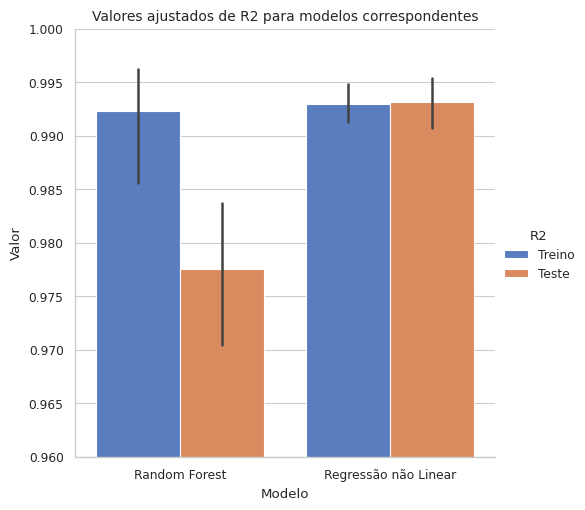
\includegraphics[width=\textwidth,height=3.125in]{compare.png}
\caption{Cada coluna representa a distribuição dos valores ajustados de
um modelo e conjunto (treino ou teste) para predição das variáveis
dinâmicas. É possível observar que ambos modelos aprendem os dados do
conjunto de treinamento, mas o modelo de Regressão não Linear alcança
uma generalização levemente melhor.}
\end{figure}

\subsubsection{Importância de Features em Random
Forests}\label{importuxe2ncia-de-features-em-random-forests}

Análise das features mais importantes foi feita para ambas variáveis
resposta e diferentes métodos de inicialização, demarcados de acordo com
as cores. As features estão ordenadas de forma descendente no gráfico
por importância média. É importante notar a diluição da importância das
features no Tempo de Consenso, em que há uma grande distinção entre
importância para cada inicialização diferente. Já na Frequência de Troca
de Opinião, a Variância do Grau e Entropia são dominantes para todas
inicializações. De forma contrária, \emph{Eigenvector} e Assortatividade
não demonstram nenhuma capacidade preditiva. Em todos os casos, não fica
claro quais métricas são determinantes para predição das variáveis
resposta. A análise foi realizada utilizando Random Forests.

\begin{figure}
\centering
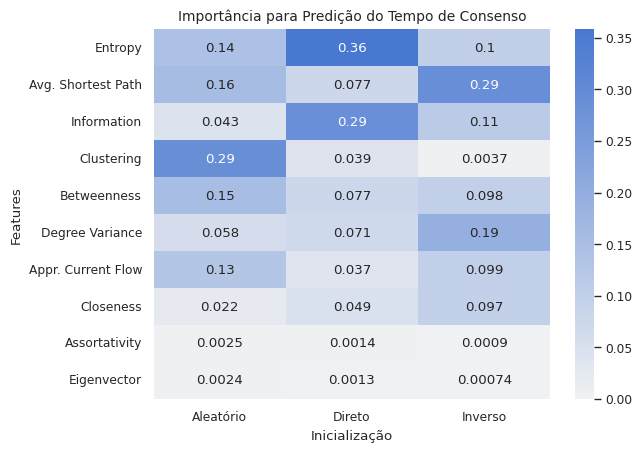
\includegraphics[width=\textwidth,height=3.70833in]{consensus_importance.png}
\caption{Importância de Features para o Tempo de Consenso: há uma
diluição de importância. \label{teste}}
\end{figure}

\begin{figure}
\centering
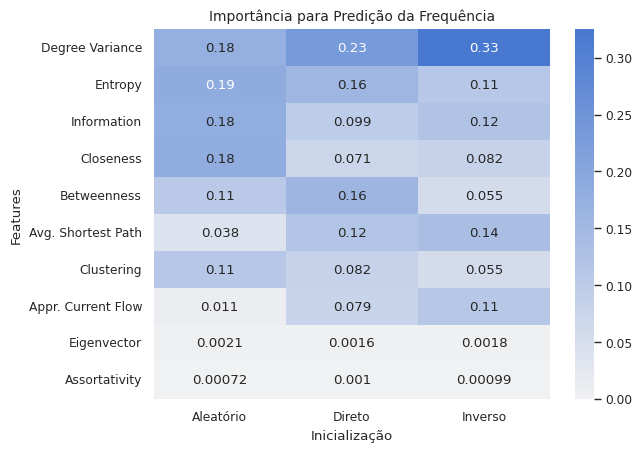
\includegraphics[width=\textwidth,height=3.70833in]{frequency_importance.png}
\caption{Importância de Features para a Frequência de Troca de Opinião:
a Variância do Grau e Entropia são dominantes.}
\end{figure}

\subsubsection{Análise das Features utilizando Regressão não Linear e
Forward
Selection}\label{anuxe1lise-das-features-utilizando-regressuxe3o-nuxe3o-linear-e-forward-selection}

Os métodos de Regressão com mínimos quadrados nos permitem aprofundar
nos resultados para maior interpretabilidade das variáveis resposta
através dos coeficientes de regressão, p-valores e outras informações.
Aqui, realizamos uma seleção empírica das variáveis das seção 2.3
prezando pela diversidade e explicabilidade. Assim, os próximos
resultados advém do mesmo cenário da subseção anterior considerando
apenas as variáveis descritas na seçao 2.3: Entropia de Shannon,
Assortatividade, \emph{Closeness Centrality} e Coeficiente de
\emph{Clustering}.

Através das tabelas obtidas para cada uma das variáveis resposta e cada
um dos métodos de inicialização percebemos através dos baixos valores de
\emph{p-value} e \emph{standard error} que há uma grande significância
das \emph{features} selecionadas. Além disso, com apenas duas features é
ppossível alcançar um coeficiente de determinação superior a \(0.98\).
No caso da Frequência de Troca de Opinião, o \emph{Clustering} se
apresenta para as três inicializações em uma relação direta: quanto
maior o coeficiente, maior a frequência de troca de opinão. É uma medida
que aumenta de acordo com o número de triângulos do total presentes na
rede. Dessa forma, é possível elaborar uma tese que a presença de
triângulos na rede incita a troca de opiniões entre os indivíduos. Para
o Tempo de Consenso, pode se observar o \emph{Closeness Centrality} em
uma relação inversa com a variável resposta. A \emph{feature} em questão
aumenta a medida que a distância média entre os pares de nós na rede
diminui. No nosso caso, isso pode indicar que quando, em média, os nós
da rede estão mais próximos uns aos outros, menor o tempo necessário
para alcançar um estado estacionário.

\begin{figure}
\centering
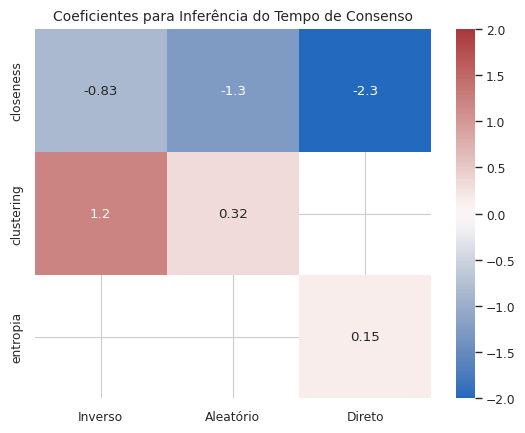
\includegraphics[width=\textwidth,height=2.66667in]{consensus_heatmap.png}
\caption{Coeficientes de Regressão obtidos para para Inferência do Tempo
de Consenso de acordo com diferentes inicializações}
\end{figure}

\begin{figure}
\centering
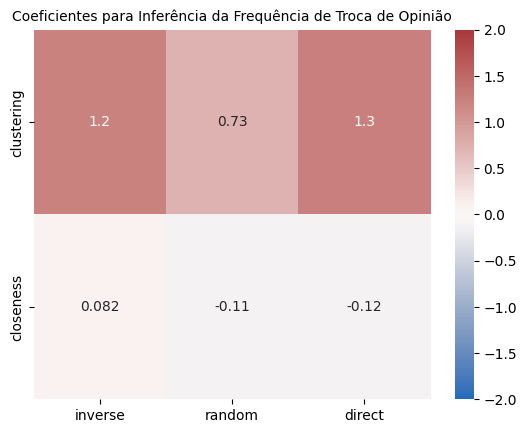
\includegraphics[width=\textwidth,height=2.66667in]{frequency_heatmap.png}
\caption{Coeficientes de Regressão obtidos para para Inferência da
Frequência de Troca de Opinião de acordo com diferentes inicializações}
\end{figure}

\section{Conclusão}\label{conclusuxe3o}

Nesse trabalho, conseguimos predizer variáveis dinâmicas associadas com
o modelo de Sznajd utilizando métricas de topologia de rede. Verificamos
que a predição obteve grande acurácia e propusemos um método para obter
maior explicabilidade e semelhante acurácia quando comparado a Random
Forests. Assim, conseguimos verificar não apenas quais \emph{features}
são mais importantes na emergência de polarização, mas também qual o
nível de influência. Principalmente, mostramos que o Coeficiente de
\emph{Clustering} e \emph{Closeness Centrality} podem ser utilizado para
predizer as variáveis dinâmicas associadas as simulações. Além disso,
três mudanças nos métodos de inicialização dos nós foram considerados,
buscando entender como as medidas topológicas podem ser influenciadas
nesse caso. Inicialmente, os nós foram escolhidos de forma aleatória,
seguindo o modelo original de Sznajd. Após, nós com maior grau foram
selecionados para investigar como seu grande número de conexões pode
influenciar a dinâmica da rede. Por fim, os nós na periferia da rede
foram selecionados para entender o impacto de agentes menos influentes.
Apesar dessas modificações impactarem o resultado das simulações,
conseguimos observar que o impacto é pequeno e as métricas selecionadas
se conservam ao longo dos experimentos.

Ao analisar a importância de features obtida a partir de experimento com
alta acurácia a partir de Random Forests, foi encontrada uma diluição de
importância, isto é, duas features tem comportamento semelhate e
impactam a regressão de maneira semelhante , o que torna a análise dos
dados mais difícil. Tal observação se confirma ao analisar o Heatmap na
figura \ref{teste}. Assim, o método proposto busca encontrar um
subconjunto de \emph{features} que obtenha alta acurácia através de
Regressão não Linear, possibilitando análise dos coeficientes. Nesse
cenário, os coeficientes de Regressão indicam que a presença de
triângulos na rede incita a troca de opiniões entre os indivíduos e que,
em média, quão menor a distância entre os nós da rede, menor o tempo
necessário para alcançar um estado estacionário. Notavelmente, a
magnitude de influência de \emph{Closeness Centrality} na predição do
Tempo de Consenso aumenta de acordo com o grau dos nós que recebem a
opinião predominante, mostrando que a proximidade entre nós é
especialmente influente quando os nós dominantes são mais conectados.

A expansão da metodologia proposta para predição e análise de variáveis
topológicas além do modelo de Sznajd pode promover novos \emph{insights}
relativos a diversos cenários e estudos em dinâmicas sociais. Trabalhos
futuros nessa direção vão contribuir para um melhor entendimento de
dinâmicas complexas para a polarização e suas implicações. A combinação
de aprendizado de máquina com redes complexas tem um grande potencial
para revolucionar nossa compreensão de sistemas sociais, levando a um
maior entendimento do comportamento e desenvolvimento de estratégias
para alcançar resultado social positivo.

\section{Referências}\label{referuxeancias}

::: \{\#refs\} :::
